\documentclass[border=10pt]{standalone}

\usepackage{tikz}
\usepackage{tikzsymbols}
\usetikzlibrary{calc,patterns,shapes.geometric}

\def\centerarc[#1](#2)(#3:#4:#5){\draw[#1] ($(#2)+({#5*cos(#3)},{#5*sin(#3)})$) arc (#3:#4:#5);}

\begin{document}
	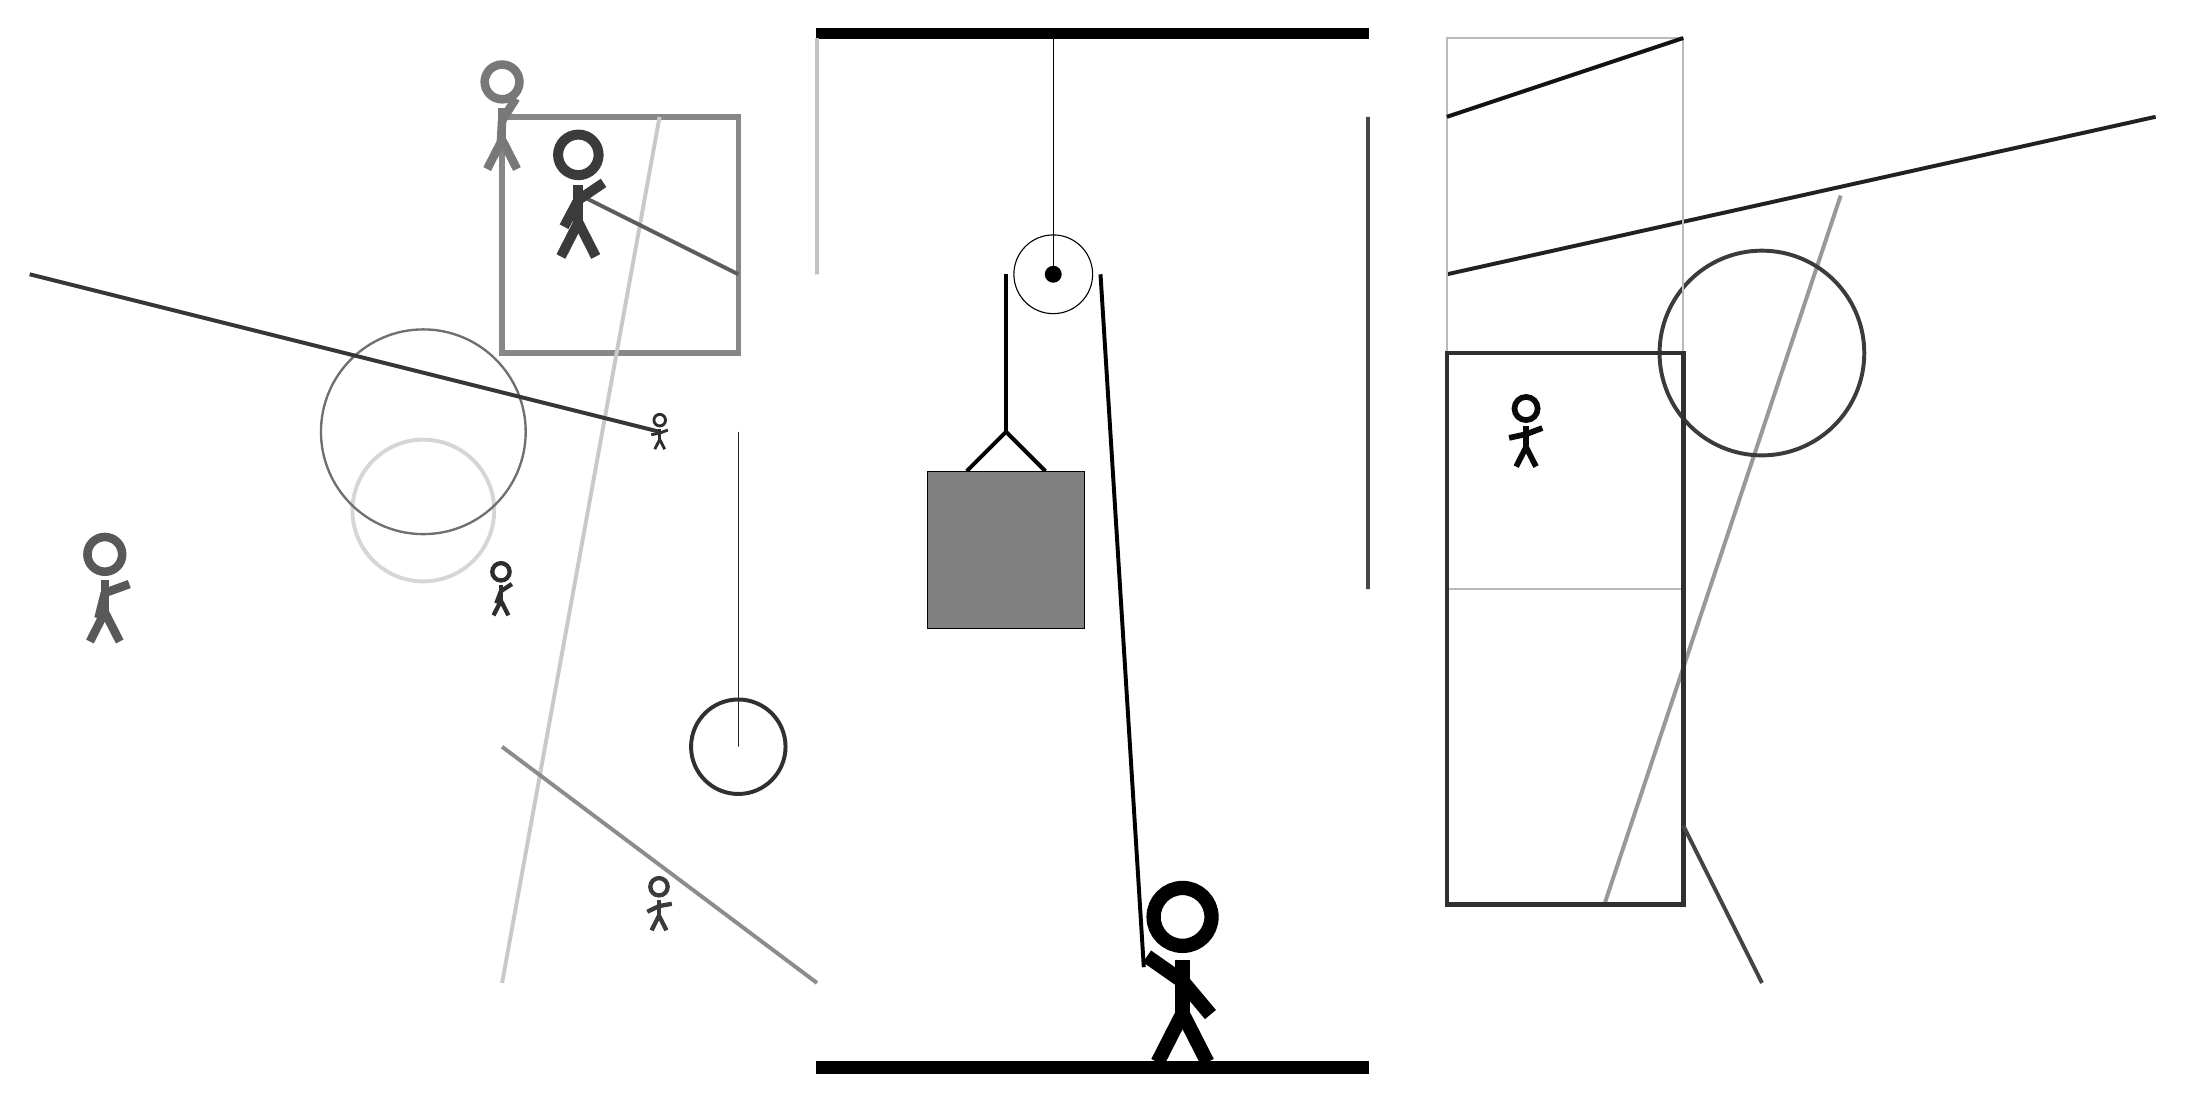
\begin{tikzpicture}
		%%%%% START %%%%%
		
		\draw[fill=black] (-2, 10) rectangle (5, 10.125);
		
		\draw (1, 7) circle (0.5);
		\draw[fill=black] (1, 7) circle (0.1);
		\draw (1, 10) -- (1, 7);
		
		\draw[line width=0.5mm] (-0.1, 4.5) -- (0.4, 5.0) -- (0.9, 4.5);
		\draw[fill=black!50] (-0.6, 4.5) rectangle (1.4, 2.5);
		
		\draw[line width=0.5mm, color=black!40](8, -1) -- (11, 8);
		
		\draw[line width=0.5mm, color=black!87](6, 7) -- (15, 9);
		\draw[line width=0.7mm, color=black!47] (-3, 6) rectangle (-6, 9);
		\draw [line width=0.5mm, color=black!16](-7, 4) circle (0.9);
		
		\draw [line width=0.3mm, color=black!56](-7, 5) circle (1.3);
		
		\draw [line width=0.5mm, color=black!77](10, 6) circle (1.3);
		
		\draw[line width=0.2mm, color=black!87] (-3, 5) rectangle (-3, 1);
		
		\node[line width=0.7mm, color=black!77] at (-4, -1) {\Strichmaxerl[3][26][10]};
		\draw[line width=0.5mm, color=black!21](-6, -2) -- (-4, 9);
		\draw[line width=0.2mm, color=black!27] (6, 3) rectangle (9, 10);
		
		\node[line width=0.3mm, color=black!65] at (-11, 3) {\Strichmaxerl[6][76][20]};
		\draw[line width=0.5mm, color=black!64](-5, 8) -- (-3, 7);
		\draw[line width=0.6mm, color=black!81] (6, -1) rectangle (9, 6);
		\draw[line width=0.5mm, color=black!93](9, 10) -- (6, 9);
		\node[line width=0.6mm, color=black!96] at (7, 5) {\Strichmaxerl[4][12][21]};
		\draw[line width=0.5mm, color=black!45](-2, -2) -- (-6, 1);
		
		\draw[line width=0.4mm, color=black!24] (-2, 7) rectangle (-2, 10);
		\draw[line width=0.5mm, color=black!72] (5, 9) rectangle (5, 3);
		\node[line width=0.3mm, color=black!82] at (-6, 3) {\Strichmaxerl[3][69][33]};
		\node[line width=0.2mm, color=black!77] at (-5, 8) {\Strichmaxerl[7][62][34]};
		\node[line width=0.5mm, color=black!53] at (-6, 9) {\Strichmaxerl[6][87][58]};
		
		\draw[line width=0.5mm, color=black!79](-4, 5) -- (-12, 7);
		\draw [line width=0.5mm, color=black!81](-3, 1) circle (0.6);
		\draw[line width=0.5mm, color=black!73](9, 0) -- (10, -2);
		\node[line width=0.4mm, color=black!82] at (-4, 5) {\Strichmaxerl[2][12][20]};
		
		
		\draw[line width=0.5mm] (0.4, 7) -- (0.4, 5.0);
		\centerarc[line width=0.5mm](1, 7)(0:180:0.6);
		\draw[line width=0.5mm](1.6, 7) -- (2.15, -1.8);
		
		\node at (2.6, -1.9) {\Strichmaxerl[10][-35][-50]};
		
		\draw[fill=black] (-2, -3) rectangle (5, -3.15);
		
		%%%%% END %%%%%
	\end{tikzpicture}
\end{document}